\documentclass[8pt]{beamer}

\usepackage[frenchb]{babel}
\usepackage[utf8x]{inputenc}
\usepackage{pifont}
\usepackage{verbatim}
\usepackage[final]{pdfpages}
\usepackage{stmaryrd}



\usetheme[secheader]{Boadilla}

\title{Distribution trouée DVWA}
\author{Florian Barbarin, Abdelkader Beldjilali, Alexis Letombe}
\date{\today}

\begin{document}

\begin{titlepage}
\begin{center}
	
\includegraphics[width=2cm]{../images/enac.png}
\end{center}
\end{titlepage}



\begin{frame}
	\tableofcontents[]
\end{frame}




\section{Introduction}

\begin{frame}
  \tableofcontents[sectionstyle=show/shaded,subsectionstyle=shaded]
\end{frame}

\begin{frame}{Introduction}



	\begin{block}{Sécurité des applications web}
		\begin{enumerate}[\ding{217}]
			\item Technologies web de plus en plus présentes, à la fois dans la vie privée et au sein des entreprises
			\item Nombreux avantages : efficacité, centralisation des données, accès facilité à l'information, etc... 
			\item Un grand nombre de menaces pèsent sur ces applications (cf. OWASP) : atteinte à la disponibilité, l'intégrité et/ou la confidentialité
		\end{enumerate}
	\end{block}
	
\begin{center}
	
\includegraphics[width=2cm]{../images/logo.jpg}
\end{center}

	\begin{block}{Présentation de l'application DVWA}
		\begin{enumerate}[\ding{217}]
			\item Application web écrite en PHP/HTML 
			\item Permet la formation à la sécurité des applications web
			\item 10 thèmes abordés
		\end{enumerate}
	\end{block}
	

\end{frame}


\section{Présentation de vulnérabilités}

\begin{frame}
  \tableofcontents[sectionstyle=show/shaded,subsectionstyle=show]
\end{frame}

\subsection{Brute Force}

\begin{frame}{Brute Force}

\begin{block}{Caractéristiques de la vulnérabilité}
	\begin{enumerate}[\ding{217}]
		\item Intervient lors de la connexion d'un utilisateur
		\item Permet la découverte du mot de passe d'un utilisateur
		\item Deux moyens de procéder : avec ou sans dictionnaire
	\end{enumerate}
\end{block}

\begin{block}{Caractéristiques de la vulnérabilité}
        \begin{enumerate}[\ding{217}]
                \item Essais à la main (sans dictionnaire)
		\item Appartition des login / mot de passe dans l'URL
		\item Essai multiples pour un login donné (si le nombre de tentatives n'est pas limité)
	\end{enumerate}
\end{block}
  
\end{frame}

\subsection{Command Injection}

\begin{frame}{Command Injection}

\begin{block}{Caractéristiques de la vulnérabilité}
	\begin{enumerate}[\ding{217}]
		\item Utilisation d'un champ prévu pour exécuter un \textit{Ping} sur l'adresse entrée
		\item Exécuter des commandes dans un champ non prévu à cet effet
		\item Possibilité d'exécuter plusieurs commandes à la suite
	\end{enumerate}
\end{block}

\begin{block}{Caractéristiques de la vulnérabilité}
	\begin{enumerate}[\ding{217}]
		\item On enchaine les commandes séparées par des ';'
		\item Naviguer dans les répertoires du système
		\item Premier point d'entrée pour une opération de plus grande ampleur
	\end{enumerate}
\end{block}

\end{frame}

\subsection{CSRF}

\begin{frame}{CSRF}

\begin{block}{Présentation de la vulnérabilité}
	\begin{enumerate}[\ding{217}]
		\item CSRF :  \textit{Cross-Site Request Forgery}
		\item Permet de modifier le mot de passe de l'utilisateur
		\item Faire exécuter une action par un utilisateur à son insu
	\end{enumerate}
\end{block}

\begin{block}{Caractéristiques de la vulnérabilité}
        \begin{enumerate}[\ding{217}]
                \item Aucune vérification de l'identité de la personne
		\item L'ingénierie sociale permet d'y arriver
		\item Un raccourcissement de l'URL qui permet l'exécution de l'action
	\end{enumerate}
\end{block}

\end{frame}

\subsection{File Inclusion}

\begin{frame}{File Inclusion}

\begin{block}{Présentation de la vulnérabilité}

\begin{center}
	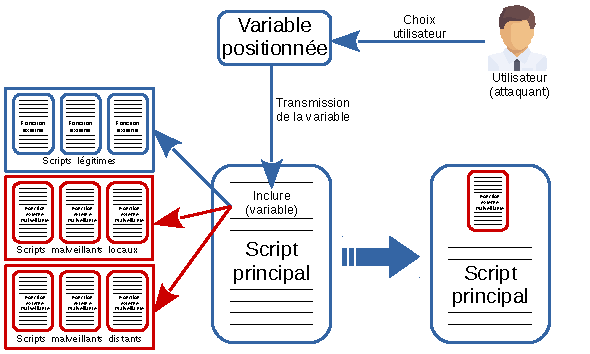
\includegraphics[scale=.8]{../images/include_hacked.pdf}
\end{center}

\end{block}

\begin{block}{Caractéristiques de la vulnérabilité}
	\begin{enumerate}[\ding{217}]
		\item Moyen d'exécuter du code
		\item Code local ou code distant
		\item Souplesse \textit{vs} sécurité
	\end{enumerate}
\end{block}

\end{frame}

\subsection{File Upload}

\begin{frame}{File Upload}


\begin{block}{Présentation de la vulnérabilité}
	\begin{enumerate}[\ding{217}]
		\item Fonctionnalité très répandue dans les applications web (\textit{cloud}, \textit{mail})
		\item Permet chargement sur le serveur de fichiers locaux
		\item Type de fichier doit être conforme à ce qu'attend l'application : contrôles nécessaires
	\end{enumerate}
\end{block}


\begin{block}{Caractéristiques de la vulnérabilité}
	\begin{enumerate}[\ding{217}]
		\item Moyen de charger sur le serveur du code malicieux
		\item Possibilité d'écraser/modifier des fichiers déjà présents sur le serveur (défacement)
		\item Mauvaise implémentation du contrôle des fichiers : ouverture du serveur à \textbf{tout} type d'attaques (scripts avec commandes systèmes, etc...)
	\end{enumerate}
\end{block}

\end{frame}

\subsection{Insecure CAPTCHA}

\begin{frame}{Insecure CAPTCHA}

\begin{block}{Présentation de la vulnérabilité}

\begin{center}
	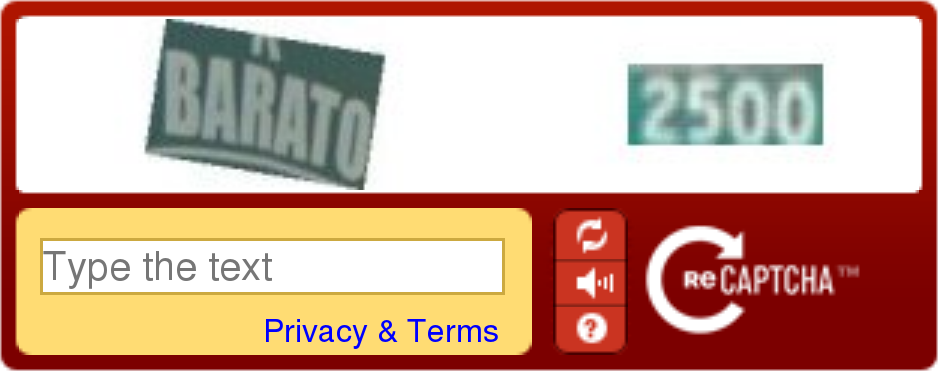
\includegraphics[scale=.15]{../images/captcha1.png}
\end{center}

	\begin{enumerate}[\ding{217}]
		\item CAPTCHA :  \textit{Completely Automated Public Turing test to tell Computers and Human Apart}
		\item Permet de décider si une action est réalisée, ou non, par un humain
		\item Éviter automatisation de certaines tâches : nécessite non-contournement du contrôle
	\end{enumerate}
\end{block}

\begin{block}{Caractéristiques de la vulnérabilité}
Vulnérabilités courantes :
	\begin{enumerate}[\ding{217}]
		\item Transmission de la solution (via URL, nom image, champ HTML caché, etc...)
		\item Mauvaise vérification de la réussite au test : contournement possible du contrôle
		\item Résolution automatique du test : contrôle doit être suffisamment difficile
	\end{enumerate}
\end{block}


\end{frame}

\subsection{Injection SQL}

\begin{frame}{Injection SQL}

\end{frame}

\subsection{Injection SQL aveugle}

\begin{frame}{Injection SQL aveugle}

\end{frame}

\subsection{Attaques Reflected XSS (non persistante)}

\begin{frame}{Attaques Reflected XSS (non persistante}

\end{frame}

\subsection{Stored XSS (persistante)}

\begin{frame}{Stored XSS (persistante)}

\end{frame}

\section{Conclusion}

\begin{frame}
  \tableofcontents[sectionstyle=show/shaded,subsectionstyle=shaded]
\end{frame}

\begin{frame}{Conclusion}

\begin{block}{Sécurité des applications web}
	\begin{enumerate}[\ding{217}]
		\item Seulement quelques vulnérabilités présentées
		\item Nombreuses autres vulnérabilités existent
		\item Sensibilité des informations échangées dans les applications web : nécessaire sécurisation
	\end{enumerate}
\end{block}

\begin{block}{Principes généraux de la sécurité des applications web}
	\begin{enumerate}[\ding{217}]
		\item Bon filtrage des saisies utilisateurs
		\item Bonne configuration du serveur web
	\end{enumerate}
\end{block}

\end{frame}
	
	
\end{document}
